\documentclass[11pt,a4paper]{article}

\usepackage[margin=1in, paperwidth=8.3in, paperheight=11.7in]{geometry}
\usepackage{amsmath,amsfonts,fancyhdr,bbm,graphicx,tikz}
\usetikzlibrary{automata,positioning}
\graphicspath{ {img/} }
\usepackage[section,nohyphen]{DomH}
\headertitle{Applied Deep Learning - Notes}

\begin{document}

\title{Applied Deep Learning - Notes}
\author{Dom Hutchinson}
\date{\today}
\maketitle

\tableofcontents\newpage

\section{Machine Learning}

\begin{definition}{Deep Representation Learning}
  \textit{Representation Learning} is a set of techniques in machine learning where a system can automatically learn representations needed for feature detection from the raw data without the need for hand-designed feature descriptions. \textit{Deep Representation Learning} is then learning to classify using this feature detection.
\end{definition}

\section{Artificial Neural Networks}

\begin{remark}{Biological Inspiration}
  In the natural world \textit{Neurons} are the basic working units of the brain. \textit{Neurons} can be split into three main areas
  \begin{enumerate}
    \item \textit{Dendrites} - Receives inputs from other neurons.
    \item \textit{Axon} - Carries information.
    \item \textit{Axon Terminals \& Synapses} = Send information to other neurons.
  \end{enumerate}
  \textit{Artificial Neural Networks} seek to mimic this structure.
\end{remark}

\begin{definition}{Neuro-Plasticity}
  \textit{Neuro-Plasticity} is the ability of a neural system to adapt its structure to accommodate new information (i.e. Learn). This can take several forms including growth \& function changes.
\end{definition}

\subsection{Feed-Forward Networks}

\begin{definition}{Feed-Forward Network} is an artificial neural network where the connections between nodes are uni-directional. Data is provided to the input layer and then an output is returned from the output layer, no layers are visited twice.

\end{definition}

\subsubsection{Perceptron}

\begin{definition}{Perceptron}
  A \textit{Perceptron} is an algorithm for supervised learning of a binary classifier. A perceptron defines a hyperplane which acts as a decision boundary which linearly separates the input-state space. These two regions correspond to the two-classes. A perceptron has the following structure.

  \begin{center}\begin{tikzpicture}
    % nodes
    \node         at (-2,0)      {$\text{bias}\big\{$};
    \node[circle] at (0,0)  (x0) {$x_0:=-1$};
    \node[circle] at (0,-1) (x1) {$x_1$};
    \node[circle] at (0,-2) (x2) {$x_2$};
    \node         at (0,-3) (x3) {$\vdots$};
    \node[circle] at (0,-4) (xk) {$x_k$};
    \node         at (0,1)       {$\overbrace{}^{\text{input}}$};

    \node[rectangle] at (3,-2) (sum) {\huge $\Sigma$};
    \node            at (3,1)       {$\overbrace{}^{\text{weighted sum}}$};
    \node[rectangle] at (6,-2) (act) {\huge $g$};
    \node            at (6,1)       {$\overbrace{}^{\text{activation function}}$};
    \node[rectangle] at (9,-2) (out) {\huge $y\in\{-1,1\}$};
    \node            at (9,1)       {$\overbrace{}^{\text{output}}$};

    % edges
    \path[->]
    (x0) edge node[above] {$w_0$} (sum)
    (x1) edge node[above] {$w_1$} (sum)
    (x2) edge node[above] {$w_2$} (sum)
    (x3) edge (sum)
    (xk) edge node[above] {$w_k$} (sum)
    (sum) edge (act)
    (act) edge (out);
  \end{tikzpicture}\end{center}
  \begin{itemize}
    \item[$x_0$] is the bias element. It is always set to $-1$ in the input and the actual value is defined by its weight $w_0$.
    \item[$\pmb{x}=(x_0,\dots,x_k)$] is the input. $(x_1,\dots,x_k)$ are the inputs for the item we wish to classify
    \item[$\pmb{w}=(w_0,\dots,w_k)$] is the weights assigned to each input.
    \item[$\Sigma$] is the weighted sum of the bias \& inputs. $\Sigma:=(\sum_{i=0}^kw_ix_i)=\pmb{w}^T\pmb{x}$
    \item[$g$] is the \textit{Activation function} which maps from $\Sigma$ to $\{-1,1\}$, effectively performing a binary classification. The user has several options for how to define this. (n.b. $g:\reals\to\{-1,1\}$)
    \item[$y$] is the output of the \textit{Activation function}. (i.e. the classification). Typically denoted as $f(\pmb{x};\pmb{w})$ \[ y=g\left(\sum_{i=0}^kx_iw_i)\right)=g(\pmb{w}^T\pmb{x})\]
  \end{itemize}
\end{definition}

\begin{remark}{Limitations of Perceptron}
  A \textit{Perceptron} can only perform linear binary classification so is not useful when two classes are not linearly separable. See \texttt{Section 2.2} for how to learn arbitrary decision boundaries.
\end{remark}

\begin{proposition}{Activation Function}
  There are several choice for the \textit{Activation Function} including:
  \begin{itemize}
    \item[\texttt{sign}] binarily assigns values depend on whether they are positive or negative.
    \[ \mathtt{sign}(x):=\begin{cases}1&x\geq0\\-1&x<0\end{cases}=\frac{x}{|x|} \]
  \end{itemize}
\end{proposition}

\begin{proposition}{Perceptron (Supervised) Learning Rule}
  We need a way for a perceptron to learn when it makes a misclassification. This is done by adjusting the weight vector $\pmb{w}$. A simple learning rule is to update the current weights by a certain proportion of the error made.
  \[ \pmb{w}_{t+1}=\pmb{w}_t+\Delta\pmb{w}\quad\text{where}\quad\Delta\pmb{w}=\begin{cases}\eta f^*(\pmb{x})\pmb{x}&\text{if }\overbrace{f^*(\pmb{x})}^\text{ground truth}\neq \overbrace{f(\pmb{x})}^\text{prediction}\\0&\text{otherwise}\end{cases}\]
  Here, $\eta\in\reals^+$ is know as the \textit{Learning Rate}. Remember that $f^*(\cdot)\in\{1,-1\}$.
\end{proposition}

\begin{proposition}{Training Process for a Single-Layer Perceptron}
  Let $\left\{\big(\pmb{x}_1,f^*(\pmb{x}_1)\big),\dots,\big(\pmb{x}_N,f^*(\pmb{x}_N)\big)\right\}$ be a set of training data. To learn a good set of weights $\pmb{w}$ do the following process.
  \begin{enumerate}
    \item Initialise the weight vector $\pmb{w}=\pmb0$
    \item Consider next training datum $\big(\pmb{x}_i,f^*(\pmb{x}_i)\big)$.
    \item Calculate prediction $f(\pmb{x})$.
    \item Compare prediction $f(\pmb{x})$ and ground truth $f^*(\pmb{x})$.
    \item Update the weight vector $\pmb{w}=\pmb{w}+\Delta\pmb{w}\quad\text{where}\quad\Delta\pmb{w}=\begin{cases}\eta f^*(\pmb{x})\pmb{x}&\text{if }f^*(\pmb{x})\neq f(\pmb{x})\\0&\text{otherwise}\end{cases}$
    \item Repeat ii)-v) until the training set is exhausted.
  \end{enumerate}
\end{proposition}

\subsubsection{Multi-Layer Perceptron}

\begin{remark}{Learning Arbitrary Decision Boundaries}
  To lean an arbitrary decision boundary (i.e. anything non-linear) can be done by using a \textit{Multi-Layer Preceptron} with non-linear activation functions.
\end{remark}

\begin{definition}{Multi-Layer Perceptron}
  A \textit{Multi-Layer Perceptron} has the same general structure as a perceptron but with multiple calculations occuring and multiple output values. Below is a diagram of a MLP of \textit{depth} $N$ (i.e. there are $N$ layers of computation)
  \begin{center}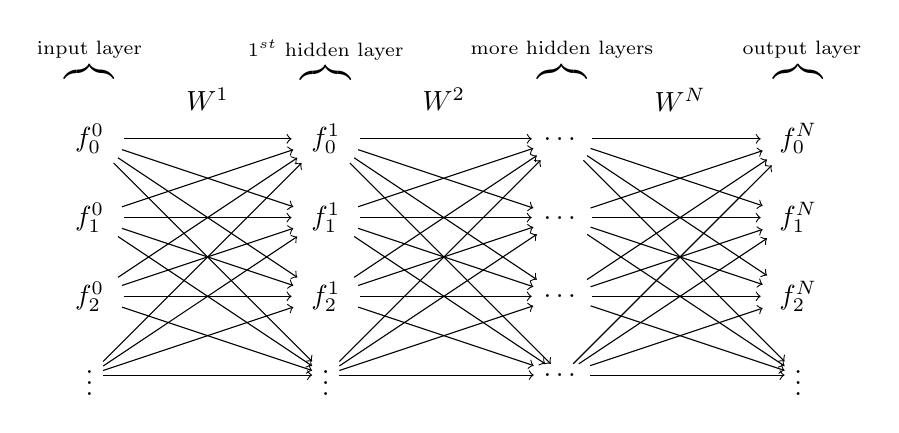
\begin{tikzpicture}
    % nodes
    \node         at (0,1)        {$\overbrace{}^{\text{input layer}}$};
    \node[circle] at (0,0)  (f00) {$f^0_0$};
    \node[circle] at (0,-1) (f01) {$f^0_1$};
    \node[circle] at (0,-2) (f02) {$f^0_2$};
    \node         at (0,-3) (f0)  {$\vdots$};
    \node         at (1.5,.5)(w1)  {$W^1$};

    \node         at (3,1)        {$\overbrace{}^{1^{st}\text{ hidden layer}}$};
    \node[circle] at (3,0)  (f10) {$f^1_0$};
    \node[circle] at (3,-1) (f11) {$f^1_1$};
    \node[circle] at (3,-2) (f12) {$f^1_2$};
    \node         at (3,-3) (f1)  {$\vdots$};
    \node         at (4.5,.5)(w2)  {$W^2$};

    \node         at (6,1)        {$\overbrace{}^\text{more hidden layers}$};
    \node[circle] at (6,0)  (f20) {$\dots$};
    \node[circle] at (6,-1) (f21) {$\dots$};
    \node[circle] at (6,-2) (f22) {$\dots$};
    \node         at (6,-3) (f2)  {$\dots$};
    \node         at (7.5,.5)(wN)  {$W^N$};

    \node         at (9,1)        {$\overbrace{}^{\text{ output layer}}$};
    \node[circle] at (9,0)  (fN0) {$f^N_0$};
    \node[circle] at (9,-1) (fN1) {$f^N_1$};
    \node[circle] at (9,-2) (fN2) {$f^N_2$};
    \node         at (9,-3) (fN)  {$\vdots$};

    % edges
    \path[->]
    % input layer
    (f00) edge (f10)
    (f00) edge (f11)
    (f00) edge (f12)
    (f00) edge (f1)

    (f01) edge (f10)
    (f01) edge (f11)
    (f01) edge (f12)
    (f01) edge (f1)

    (f02) edge (f10)
    (f02) edge (f11)
    (f02) edge (f12)
    (f02) edge (f1)

    (f0) edge (f10)
    (f0) edge (f11)
    (f0) edge (f12)
    (f0) edge (f1)
    % first hidden layer
    (f10) edge (f20)
    (f10) edge (f21)
    (f10) edge (f22)
    (f10) edge (f2)

    (f11) edge (f20)
    (f11) edge (f21)
    (f11) edge (f22)
    (f11) edge (f2)

    (f12) edge (f20)
    (f12) edge (f21)
    (f12) edge (f22)
    (f12) edge (f2)

    (f1) edge (f20)
    (f1) edge (f21)
    (f1) edge (f22)
    (f1) edge (f2)

    % output layer
    (f20) edge (fN0)
    (f20) edge (fN1)
    (f20) edge (fN2)
    (f20) edge (fN)

    (f21) edge (fN0)
    (f21) edge (fN1)
    (f21) edge (fN2)
    (f21) edge (fN)

    (f22) edge (fN0)
    (f22) edge (fN1)
    (f22) edge (fN2)
    (f22) edge (fN)

    (f2) edge (fN0)
    (f2) edge (fN1)
    (f2) edge (fN2)
    (f2) edge (fN)
    ;

  \end{tikzpicture}\end{center}
  Note that each layer can have a different \textit{width} (i.e. number of nodes in the layer). For each consecutive pair of layers $\pmb{f}^i,\pmb{f}^j$ (of widths $n_i,n_j$ respectively) there is an associated weight matrix $W\in\reals^{n_i\times n_j}$ st $\pmb{f}^j=W^T\pmb{f}^i$.
  \var The values from the output layer are then passed to an \textit{activation function} to make a classification. %TODO verify this
\end{definition}

\begin{remark}{Using MLPs}
  An MLP with a \textit{single} hidden layer is sufficient to represent any boolean or continuous function, althought the layer may be exponentially wider than the input.
  \par An MPL with \textit{two} hidden layers is sufficient to represent any mathematical function.
\end{remark}

\begin{proposition}{MLPs as Computation Graphs}
  \[\begin{array}{rrrll}
    &s_i^j&:=&(W^j)^Tf^{j-1}&\tiny \text{weighted sum of the }i^{th}\text{ node of the }j^{th}\text{ hidden layer}\\
    \implies&\dfrac{\partial s_i^j}{\partial w_{ii}^j}&=&f_i^{j-1}\\
    &f_i^j&:=&g_i^j(s_i^j)&\tiny i^{th}\text{ output vajue of }j^{th}\text{ hidden layer}\\
    \implies&\dfrac{\partial f_i^j}{\partial s_i^j}&=&\text{depends on def of }g_i^j
  \end{array}\]

\end{proposition}

\section{Training Algorithms}

\begin{definition}{Cost/Loss Function, $J$}
  A \textit{Cost Function} $J(\cdot;\cdot)$ is a real-valued measure of how inaccurate a classifier is for a given input configuration (test data \& weights). Greater values imply the classifier is less accurate. Here are some common cost functions
  \begin{itemize}
    \item[Expected Loss] $\displaystyle J(X;\pmb{w})=\expect[L(f(\pmb{x},\pmb{w}),f^*(\pmb{x}))]$
    \item[Empirical Risk] $\displaystyle J(X;\pmb{w})=\frac1{|X|}\sum_{\pmb{x}\in X}L(f(\pmb{x},\pmb{w}),f^*(\pmb{x}))$
  \end{itemize}
  Here $L(x,x^*)$ is a measure of loss (distance) between two values. This is defined by the user on a case by case basis. Popular definitions are: $|x-x^*|,\ (x-x^*)^2$ \& $\indexed\{x=x^*\}$
\end{definition}

\subsection{Gradient Descent}

\begin{definition}{Gradient Descent}
  \textit{Gradient Descent} aims to learn a set of weight values $\pmb{w}$ which produce a local minimum for a given cost function $J$. The update rule for gradient descent is
  \[ \pmb{w}_{t+1}=\pmb{w}_t-\underbrace{\eta\cdot\nabla J(X;\pmb{w}_t)}_{\Delta\pmb{w}} \]
  $\nabla J(X;\pmb{w}_t)$ is the partial derivative of the cost function wrt to the weights and gives the direction of the greatest descent. We can calculate the $i^\text{th}$ component of $\Delta\pmb{w}$ after observing $(\pmb{x},f^*(\pmb{x}))$
  \[ [\Delta\pmb{w}]_i=\eta x_i(\underbrace{\pmb{w}^T_t\pmb{x}}_{f(\pmb{x};\pmb{w}_t)}-f^*(\pmb{x})) \]
\end{definition}

\subsubsection{Auto-Differentitation}

\begin{proposition}{Calculating Partial Derivatives}
  There are three ways to calculate the partial derivatives required for \textit{Gradient Descent}.
  \begin{itemize}
    \item \textit{Symbolic Differentiation} (i.e. algebra). Hard to define to work in all cases.
    \item \textit{Numerical Differentiation} (i.e. check values in a neighbourhood and approximate the best direction). Easy to implement but low accuracy and high computational cost.
    \item \textit{Automatic-Differentiation} using feedforward computation graphs. See below
  \end{itemize}
\end{proposition}

\begin{definition}{Feedforward Computational Graph}
  Given a series of equations we can construct a \textit{feedforward computational graph}. \textit{Feedforward computational graphs} have a node for each variable or constant, and then an edge between nodes which are dependent. Once values are defined for all variables at a given depth, values can easily be calculated for variables higher up the tree.
\end{definition}

\begin{example}{Feedforward Computational Graph}
  Consider the following series of equations
  \[\begin{array}{rclcrcl}
    a&=&b\times c&\quad&b&=&d+e\\
    c&=&e+2&&d&=&3+f\\
    e&=&f\times g
  \end{array}\]
  We can construct the following \textit{Computational Graph}
  \begin{center}\begin{tikzpicture}
    % nodes
    \node[circle] at (0,0)   (3) {$3$};
    \node[circle] at (0,-2)  (f) {$f$};
    \node[circle] at (0,-4)  (g) {$g$};

    \node[circle] at (2,-1)  (d) {$d=3+f$};
    \node[circle] at (2,-3)  (e) {$e=f\times g$};
    \node[circle] at (2,-5)  (2) {$2$};

    \node[circle] at (4,-2)  (b) {$b=d+e$};
    \node[circle] at (4,-4)  (c) {$c=e+2$};

    \node[circle] at (6,-3)  (a) {$a=b\times c$};

    % edges
    \path[->]
    (3) edge (d)
    (f) edge (d)
    (f) edge (e)
    (g) edge (e)

    (d) edge (b)
    (e) edge (b)
    (e) edge (c)
    (2) edge (c)

    (b) edge (a)
    (c) edge (a)
    ;
  \end{tikzpicture}\end{center}
\end{example}

\begin{definition}{Auto-Differentiation using a Feedforward Computational Graph}
  Consider two nodes in a computational graph $x,y$ and suppose you want to find the partial derivative $\frac{\partial x}{\partial y}$.
  \begin{enumerate}
    \item Establish all the paths from $y$ to $x$ in the graph.
    \item Calculate the partial derivatives of each step of these graphs. (i.e. if there is a path $y\to a\to x$ calculate $\frac{\partial a}{\partial y},\frac{\partial x}{\partial a}$).
    \item Apply the chain rule along each path (i.e. For $y\to a\to x$ calculate $\frac{\partial a}{\partial y}\cdot\frac{\partial x}{\partial a}$).
    \item Sum these calculations together to get the final result $\frac{\partial x}{\partial y}$.
    \item Substitute variables to make computation easier.
  \end{enumerate}
\end{definition}

\begin{example}{Auto-Differentiation using a Feedforward Computational Graph}
  Consider the graph in \texttt{Example 3.1} and wanting to calculate $\frac{\partial f}{\partial a}$.
  \begin{enumerate}
    \item There are three paths from $f$ to $a$ in the graph: (1) $f\to d\to b\to a$; (2) $f\to e\to b\to a$; and, (3) $f\to e\to c\to a$.
    \item We need to calculate the following partial derivatives: $\frac{\partial d}{\partial f},\frac{\partial b}{\partial d},\frac{\partial a}{\partial b}$ for (1); $\frac{\partial e}{\partial f},\frac{\partial b}{\partial e},\frac{\partial a}{\partial b}$ for (2); and, $\frac{\partial e}{\partial f},\frac{\partial c}{\partial e},\frac{\partial a}{\partial c}$ for (3).
    \[\begin{array}{rclcrclcrcl}
      &(1)&&&&(2)&&&&(3)\\
      \frac{\partial d}{\partial f}&=&1&\quad&\frac{\partial e}{\partial f}&=&g&\quad&\frac{\partial e}{\partial f}&=&g\\
      \frac{\partial b}{\partial d}&=&1&\quad&\frac{\partial b}{\partial e}&=&1&\quad&\frac{\partial c}{\partial e}&=&1\\
      \frac{\partial a}{\partial b}&=&c&\quad&\frac{\partial a}{\partial b}&=&c&\quad&\frac{\partial a}{\partial c}&=&b
    \end{array}\]
    \item Applying the chain rule to each path gives
    \[\begin{array}{rrcl}
      (1)&\frac{\partial d}{\partial f}\frac{\partial b}{\partial d}\frac{\partial a}{\partial b}&=&1\cdot1\cdot c=c\\
      (2)&\frac{\partial e}{\partial f}\frac{\partial e}{\partial f}\frac{\partial b}{\partial e}&=&g\cdot1\cdot1\cdot c=gc\\
      (3)&\frac{\partial e}{\partial f}\frac{\partial c}{\partial e}\frac{\partial a}{\partial c}&=&g\cdot1\cdot b=gb\\
    \end{array}\]
    \item Summing the terms together we get
    \[ \frac{\partial a}{\partial f}=c+gc+gb \]
    \item By substitution we get a final expression
    \[ \frac{\partial a}{\partial f}=2+5g+2fg+2fg^2 \]
  \end{enumerate}
  So when $f=4,g=2$ we have that $a=150$ and $\frac{\partial a}{\partial f}=60$.
\end{example}


\end{document}
